% !TEX root = ./main.tex
\graphicspath{{figures_SD7003/}}% Set graphics path location

\subsection{SD7003 airfoil at 4$\degr$ angle of attack}
From Williams's thesis\cite{williams2013thesis}

\begin{table}[H]
\centering
\begin{tabular}{ l| l l| l l| l l} 
  
 &  \multicolumn{2}{|c|}{$Re = 10K$}  & \multicolumn{2}{|c|}{$Re = 22K$} & \multicolumn{2}{|c}{$Re = 22K$}  \\ 
 Source & $C_L$ & $C_D$ & $C_L$ & $C_D$ & $C_L$ & $C_D$   \\ 
\hline
 Uranga et al.\cite{uranga2011implicit} & 0.3755 & 0.04978 & 0.6707 & 0.04510 & 0.5730 & 0.02097  \\ 
$c_{dg},\kappa_{dg}$ & 0.3719 & 0.04940 & 0.6722 & 0.04295 & 0.5831 & 0.01975 \\ 
$c_{+},\kappa_{+}$ & 0.3713 & 0.04935 & 0.6655 & 0.04275 & 0.5774 & 0.02005  \\ 
 \end{tabular}
\caption{Time-averaged values of the lift and drag coefficients for the SD7003 airfoil flows with $Re = 10000, 22000, 60000$}
\label{table:sdAirfoilForce} 
 \end{table}


%\begin{figure}
%\centering
%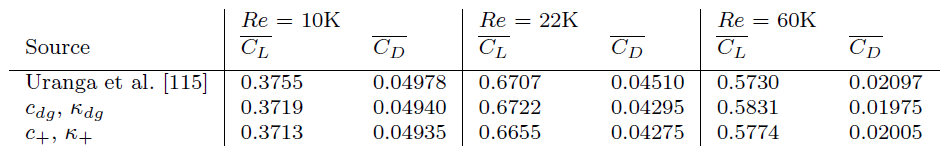
\includegraphics[height=30mm]{table_926} \\
%\caption{Time-averaged values of the lift and drag coefficients for the SD7003 airfoil flows with $Re = 10000, 22000, 60000$}
%\label{fig:table_926}
%\end{figure}

\begin{figure}
\centering
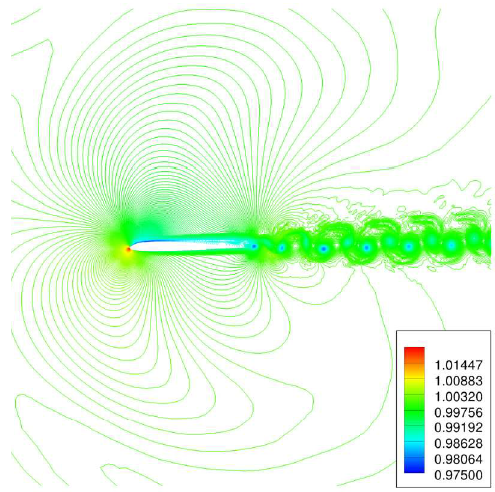
\includegraphics[height=60mm]{figure_935a} \\
\caption{Density contour for the flow with $Re = 10000$ around the SD7003 airfoil.}
\label{fig:figure_935a}
\end{figure}

\begin{figure}
\centering
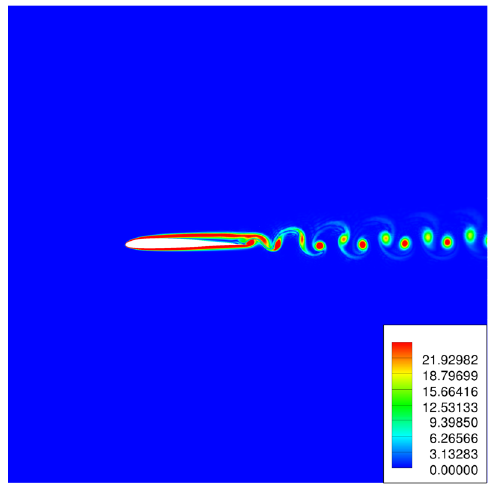
\includegraphics[height=60mm]{figure_935b} \\
\caption{Vorticity contour for the flow with $Re = 10000$ around the SD7003 airfoil.}
\label{fig:figure_935b}
\end{figure}

\begin{figure}
\centering
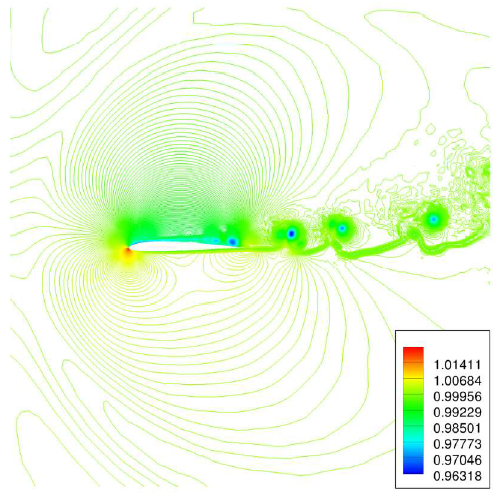
\includegraphics[height=60mm]{figure_936a} \\
\caption{Density contour for the flow with $Re = 22000$ around the SD7003 airfoil.}
\label{fig:figure_936a}
\end{figure}

\begin{figure}
\centering
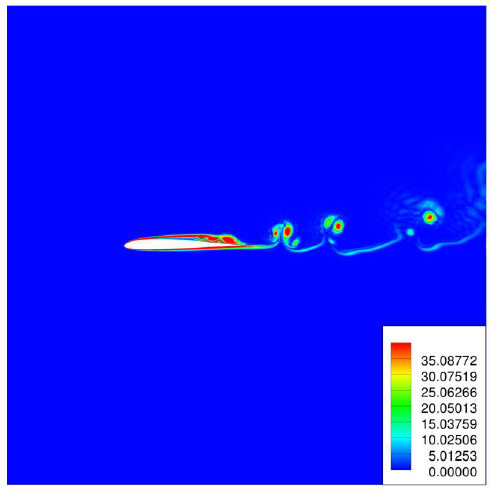
\includegraphics[height=60mm]{figure_936b} \\
\caption{Vorticity contour for the flow with $Re = 22000$ around the SD7003 airfoil.}
\label{fig:figure_936b}
\end{figure}

\begin{figure}
\centering
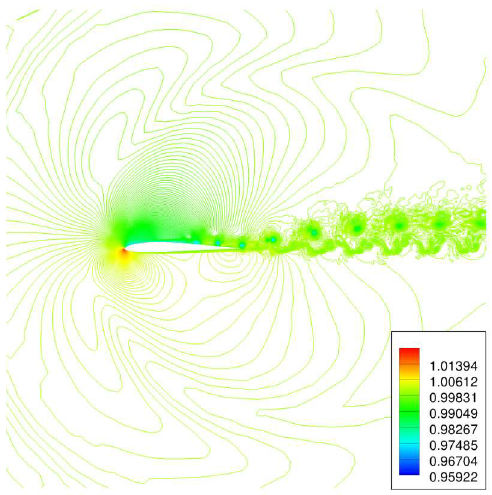
\includegraphics[height=60mm]{figure_937a} \\
\caption{Density contour for the flow with $Re = 60000$ around the SD7003 airfoil.}
\label{fig:figure_937a}
\end{figure}

\begin{figure}
\centering
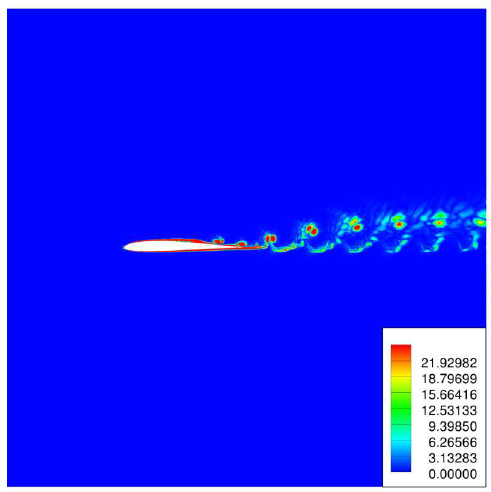
\includegraphics[height=60mm]{figure_937b} \\
\caption{Vorticity contour for the flow with $Re = 60000$ around the SD7003 airfoil.}
\label{fig:figure_937b}
\end{figure}


\subsection{SD7003 wing section at 4$\degr$ angle of attack}
From David's thesis.
%\subsubsection{Laminar Flow around a Delta Wing}

\begin{table}[H]
\centering
\begin{tabular}{ l| l l| l l| l l} 
  
 &  \multicolumn{2}{|c|}{$Re = 10K$}  \\ 
 Source & $C_L$ & $C_D$    \\ 
\hline
 Uranga et al.\cite{uranga2011implicit} & 0.3755 & 0.04978   \\ 
$c_{dg},\kappa_{dg}$ & 0.3719 & 0.04940  \\ 
$c_{+},\kappa_{+}$ & 0.3713 & 0.04935 \\ 
 \end{tabular}
\caption{Time-averaged values of the lift and drag coefficients for the SD7003 wing-section in a flow with $Re = 10000$}
\label{table:sdWingForce} 
 \end{table}

\begin{figure}
\centering
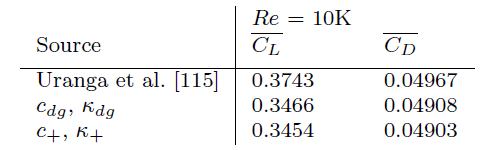
\includegraphics[height=20mm]{table_927} \\
\caption{Time-averaged values of the lift and drag coefficients for the SD7003 wing-section in a flow with $Re = 10000$}
\label{fig:table_927}
\end{figure}

\begin{figure}
\centering
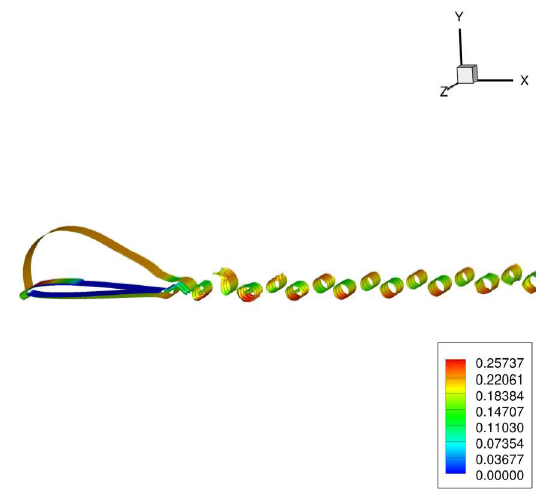
\includegraphics[height=60mm]{figure_939a} \\
\caption{Density isosurfaces colored by Mach number for the flow with $Re = 10000$ around the SD7003 wing-section.}
\label{fig:figure_939a}
\end{figure}

\begin{figure}
\centering
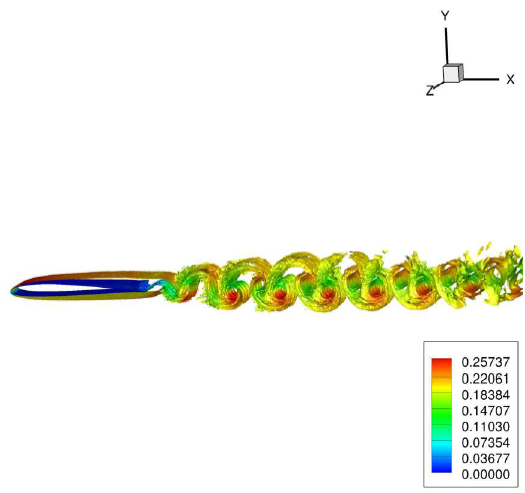
\includegraphics[height=60mm]{figure_939b} \\
\caption{Vorticity isosurfaces colored by Mach number for the flow with $Re = 10000$ around the SD7003 wing-section.}
\label{fig:figure_939b}
\end{figure}
\newpage
